\documentclass[tikz,border=0pt]{standalone}
\usepackage{xcolor}
% Palette: Sam_Comm_final.png by eye (as Pursuer's art.py), and Gatecrasher's own.
\definecolor{ink}{HTML}{3B2340}
\definecolor{sky}{HTML}{EFC46A}
\definecolor{skyhi}{HTML}{F5DA92}
\definecolor{skylow}{HTML}{E9B060}
\definecolor{cloud}{HTML}{F2D58A}
\definecolor{wallA}{HTML}{E88A73}
\definecolor{wallB}{HTML}{EE9F7E}
\definecolor{wallC}{HTML}{E47A7E}
\definecolor{wallD}{HTML}{F0B07E}
\definecolor{wallE}{HTML}{D9765F}
\definecolor{wallF}{HTML}{E99A8A}
\definecolor{greenA}{HTML}{8DBB7E}
\definecolor{greenB}{HTML}{6FA77A}
\definecolor{greenC}{HTML}{A9C97F}
\definecolor{greenD}{HTML}{5E9C6A}
\definecolor{window}{HTML}{F6E7A0}
\definecolor{windark}{HTML}{8C5A64}
\definecolor{metal}{HTML}{8D9A93}
\definecolor{metaldark}{HTML}{5E6B66}
\definecolor{wood}{HTML}{B9835A}
\definecolor{paving}{HTML}{E2BD8C}
\definecolor{ground}{HTML}{D3A77D}
\definecolor{stone}{HTML}{E7C9A0}
\definecolor{paper}{HTML}{F6E7C4}
\definecolor{cardboard}{HTML}{C9A06A}
\definecolor{cardboarddark}{HTML}{A47C4C}
\definecolor{red}{HTML}{B3262E}
\definecolor{eyewhite}{HTML}{FBF4E4}
\definecolor{skin}{HTML}{E8B07C}
\definecolor{skinB}{HTML}{C98B5E}
\definecolor{skinC}{HTML}{F2C9A0}
\definecolor{hairdark}{HTML}{2A1E33}
\definecolor{hairred}{HTML}{A8553A}
\definecolor{leather}{HTML}{33293D}
\definecolor{chrome}{HTML}{C9D3CF}
\definecolor{chromedark}{HTML}{7F8C88}
\definecolor{glass}{HTML}{A9D4CB}
\definecolor{lamp}{HTML}{FFE6A3}
\definecolor{smoke}{HTML}{E8D3AE}
\definecolor{shingle}{HTML}{C9604F}
\definecolor{gold}{HTML}{F2B53A}
\definecolor{portalblue}{HTML}{2FA8E8}
\definecolor{portalbluehi}{HTML}{A6DDF5}
\definecolor{portalorange}{HTML}{F2812E}
\definecolor{portalorangehi}{HTML}{F9C891}
\definecolor{olive}{HTML}{7A8450}
\definecolor{olivedark}{HTML}{5C6539}
\definecolor{khaki}{HTML}{C2A66E}
\definecolor{khakidark}{HTML}{9E8350}
\definecolor{mule}{HTML}{9A6A44}
\definecolor{muledark}{HTML}{6B4730}
\definecolor{mulelight}{HTML}{C99A6E}
\definecolor{bandana}{HTML}{C8343A}
\definecolor{suit}{HTML}{56704F}
\definecolor{camoA}{HTML}{8DA867}
\definecolor{camoB}{HTML}{3B5240}
\definecolor{lens}{HTML}{8EF0C6}
\definecolor{lenshi}{HTML}{E2FFF2}
\definecolor{sea}{HTML}{5FB3B0}
\definecolor{seahi}{HTML}{8FCFC0}
\definecolor{seadark}{HTML}{3F8F92}
\definecolor{concrete}{HTML}{E6C29A}
\definecolor{concretedark}{HTML}{C9A07A}
\definecolor{heli}{HTML}{4F8F86}
\definecolor{helidark}{HTML}{3A6C66}
\definecolor{duskA}{HTML}{7A5272}
\definecolor{duskB}{HTML}{B06A78}
\definecolor{duskC}{HTML}{DE8E72}
\definecolor{dirt}{HTML}{C08A68}
\definecolor{dirtdark}{HTML}{A87256}
\definecolor{beam}{HTML}{FFF3BE}
\definecolor{sunA}{HTML}{F3B86A}
\definecolor{sunB}{HTML}{EE9268}
\definecolor{sunC}{HTML}{E57766}
\definecolor{sundisc}{HTML}{FBE3A0}
\definecolor{seadusk}{HTML}{6F9E9C}
\definecolor{balloon}{HTML}{F8F0DE}
\definecolor{hay}{HTML}{E9C46A}
\definecolor{haydark}{HTML}{C99B45}
\definecolor{barn}{HTML}{C9604F}
\definecolor{trim}{HTML}{F6E7C4}
\begin{document}
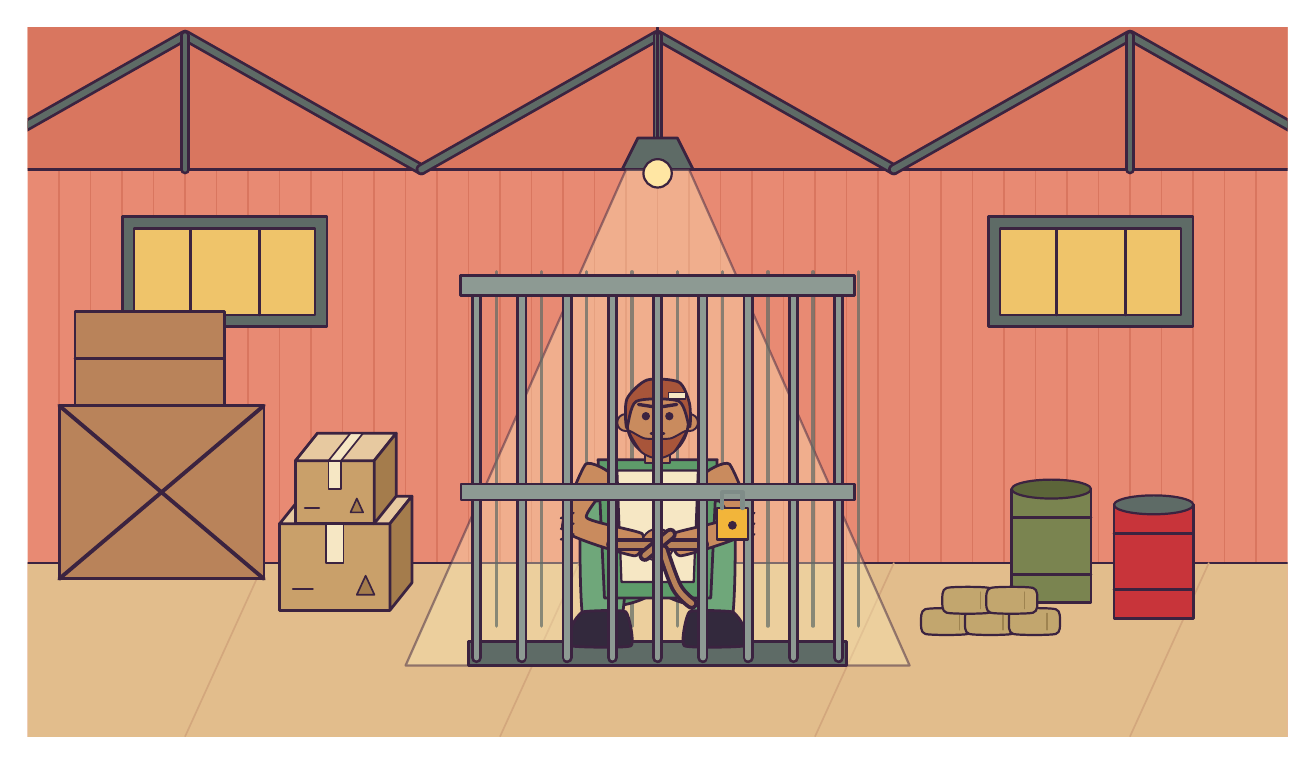
\begin{tikzpicture}
\useasboundingbox (0,0) rectangle (16,9);
\clip (0,0) rectangle (16,9);
\filldraw[draw=ink, line width=1pt, line join=round, fill=wallA] (-0.2,-0.2) -- (16.2,-0.2) -- (16.2,9.2) -- (-0.2,9.2) -- cycle;
\draw[wallE, line width=0.5pt, line cap=round, line join=round] (0.4,2.2) -- (0.4,7.2);
\draw[wallE, line width=0.5pt, line cap=round, line join=round] (0.8,2.2) -- (0.8,7.2);
\draw[wallE, line width=0.5pt, line cap=round, line join=round] (1.2,2.2) -- (1.2,7.2);
\draw[wallE, line width=0.5pt, line cap=round, line join=round] (1.6,2.2) -- (1.6,7.2);
\draw[wallE, line width=0.5pt, line cap=round, line join=round] (2,2.2) -- (2,7.2);
\draw[wallE, line width=0.5pt, line cap=round, line join=round] (2.4,2.2) -- (2.4,7.2);
\draw[wallE, line width=0.5pt, line cap=round, line join=round] (2.8,2.2) -- (2.8,7.2);
\draw[wallE, line width=0.5pt, line cap=round, line join=round] (3.2,2.2) -- (3.2,7.2);
\draw[wallE, line width=0.5pt, line cap=round, line join=round] (3.6,2.2) -- (3.6,7.2);
\draw[wallE, line width=0.5pt, line cap=round, line join=round] (4,2.2) -- (4,7.2);
\draw[wallE, line width=0.5pt, line cap=round, line join=round] (4.4,2.2) -- (4.4,7.2);
\draw[wallE, line width=0.5pt, line cap=round, line join=round] (4.8,2.2) -- (4.8,7.2);
\draw[wallE, line width=0.5pt, line cap=round, line join=round] (5.2,2.2) -- (5.2,7.2);
\draw[wallE, line width=0.5pt, line cap=round, line join=round] (5.6,2.2) -- (5.6,7.2);
\draw[wallE, line width=0.5pt, line cap=round, line join=round] (6,2.2) -- (6,7.2);
\draw[wallE, line width=0.5pt, line cap=round, line join=round] (6.4,2.2) -- (6.4,7.2);
\draw[wallE, line width=0.5pt, line cap=round, line join=round] (6.8,2.2) -- (6.8,7.2);
\draw[wallE, line width=0.5pt, line cap=round, line join=round] (7.2,2.2) -- (7.2,7.2);
\draw[wallE, line width=0.5pt, line cap=round, line join=round] (7.6,2.2) -- (7.6,7.2);
\draw[wallE, line width=0.5pt, line cap=round, line join=round] (8,2.2) -- (8,7.2);
\draw[wallE, line width=0.5pt, line cap=round, line join=round] (8.4,2.2) -- (8.4,7.2);
\draw[wallE, line width=0.5pt, line cap=round, line join=round] (8.8,2.2) -- (8.8,7.2);
\draw[wallE, line width=0.5pt, line cap=round, line join=round] (9.2,2.2) -- (9.2,7.2);
\draw[wallE, line width=0.5pt, line cap=round, line join=round] (9.6,2.2) -- (9.6,7.2);
\draw[wallE, line width=0.5pt, line cap=round, line join=round] (10,2.2) -- (10,7.2);
\draw[wallE, line width=0.5pt, line cap=round, line join=round] (10.4,2.2) -- (10.4,7.2);
\draw[wallE, line width=0.5pt, line cap=round, line join=round] (10.8,2.2) -- (10.8,7.2);
\draw[wallE, line width=0.5pt, line cap=round, line join=round] (11.2,2.2) -- (11.2,7.2);
\draw[wallE, line width=0.5pt, line cap=round, line join=round] (11.6,2.2) -- (11.6,7.2);
\draw[wallE, line width=0.5pt, line cap=round, line join=round] (12,2.2) -- (12,7.2);
\draw[wallE, line width=0.5pt, line cap=round, line join=round] (12.4,2.2) -- (12.4,7.2);
\draw[wallE, line width=0.5pt, line cap=round, line join=round] (12.8,2.2) -- (12.8,7.2);
\draw[wallE, line width=0.5pt, line cap=round, line join=round] (13.2,2.2) -- (13.2,7.2);
\draw[wallE, line width=0.5pt, line cap=round, line join=round] (13.6,2.2) -- (13.6,7.2);
\draw[wallE, line width=0.5pt, line cap=round, line join=round] (14,2.2) -- (14,7.2);
\draw[wallE, line width=0.5pt, line cap=round, line join=round] (14.4,2.2) -- (14.4,7.2);
\draw[wallE, line width=0.5pt, line cap=round, line join=round] (14.8,2.2) -- (14.8,7.2);
\draw[wallE, line width=0.5pt, line cap=round, line join=round] (15.2,2.2) -- (15.2,7.2);
\draw[wallE, line width=0.5pt, line cap=round, line join=round] (15.6,2.2) -- (15.6,7.2);
\filldraw[draw=ink, line width=1pt, line join=round, fill=wallE] (-0.2,7.2) -- (16.2,7.2) -- (16.2,9.2) -- (-0.2,9.2) -- cycle;
\draw[ink, line width=4.2pt, line cap=round, line join=round] (-1,7.2) -- (2,8.9) -- (5,7.2);
\draw[metaldark, line width=2.2pt, line cap=round, line join=round] (-1,7.2) -- (2,8.9) -- (5,7.2);
\draw[ink, line width=3.6pt, line cap=round, line join=round] (2,7.2) -- (2,8.9);
\draw[metaldark, line width=1.6pt, line cap=round, line join=round] (2,7.2) -- (2,8.9);
\draw[ink, line width=4.2pt, line cap=round, line join=round] (5,7.2) -- (8,8.9) -- (11,7.2);
\draw[metaldark, line width=2.2pt, line cap=round, line join=round] (5,7.2) -- (8,8.9) -- (11,7.2);
\draw[ink, line width=3.6pt, line cap=round, line join=round] (8,7.2) -- (8,8.9);
\draw[metaldark, line width=1.6pt, line cap=round, line join=round] (8,7.2) -- (8,8.9);
\draw[ink, line width=4.2pt, line cap=round, line join=round] (11,7.2) -- (14,8.9) -- (17,7.2);
\draw[metaldark, line width=2.2pt, line cap=round, line join=round] (11,7.2) -- (14,8.9) -- (17,7.2);
\draw[ink, line width=3.6pt, line cap=round, line join=round] (14,7.2) -- (14,8.9);
\draw[metaldark, line width=1.6pt, line cap=round, line join=round] (14,7.2) -- (14,8.9);
\filldraw[draw=ink, line width=1pt, line join=round, fill=metaldark] (1.2,5.2) -- (3.8,5.2) -- (3.8,6.6) -- (1.2,6.6) -- cycle;
\filldraw[draw=ink, line width=0.8pt, line join=round, fill=sky] (1.35,5.35) -- (3.65,5.35) -- (3.65,6.45) -- (1.35,6.45) -- cycle;
\draw[ink, line width=1pt, line cap=round, line join=round] (2.07,5.35) -- (2.07,6.45);
\draw[ink, line width=1pt, line cap=round, line join=round] (2.94,5.35) -- (2.94,6.45);
\filldraw[draw=ink, line width=1pt, line join=round, fill=metaldark] (12.2,5.2) -- (14.8,5.2) -- (14.8,6.6) -- (12.2,6.6) -- cycle;
\filldraw[draw=ink, line width=0.8pt, line join=round, fill=sky] (12.35,5.35) -- (14.65,5.35) -- (14.65,6.45) -- (12.35,6.45) -- cycle;
\draw[ink, line width=1pt, line cap=round, line join=round] (13.07,5.35) -- (13.07,6.45);
\draw[ink, line width=1pt, line cap=round, line join=round] (13.94,5.35) -- (13.94,6.45);
\filldraw[draw=ink, line width=1pt, line join=round, fill=paving] (-0.2,-0.2) -- (16.2,-0.2) -- (16.2,2.2) -- (-0.2,2.2) -- cycle;
\draw[ground, line width=0.6pt, line cap=round, line join=round] (-2,0) -- (-1,2.2);
\draw[ground, line width=0.6pt, line cap=round, line join=round] (2,0) -- (3,2.2);
\draw[ground, line width=0.6pt, line cap=round, line join=round] (6,0) -- (7,2.2);
\draw[ground, line width=0.6pt, line cap=round, line join=round] (10,0) -- (11,2.2);
\draw[ground, line width=0.6pt, line cap=round, line join=round] (14,0) -- (15,2.2);
\draw[ground, line width=0.6pt, line cap=round, line join=round] (18,0) -- (19,2.2);
\filldraw[draw=ink, line width=1pt, line join=round, fill=wood] (0.4,2) -- (3,2) -- (3,4.2) -- (0.4,4.2) -- cycle;
\draw[ink, line width=1.4pt, line cap=round, line join=round] (0.4,2) -- (3,4.2);
\draw[ink, line width=1.4pt, line cap=round, line join=round] (0.4,4.2) -- (3,2);
\filldraw[draw=ink, line width=1pt, line join=round, fill=wood] (0.6,4.2) -- (2.5,4.2) -- (2.5,5.4) -- (0.6,5.4) -- cycle;
\draw[ink, line width=1pt, line cap=round, line join=round] (0.6,4.8) -- (2.5,4.8);
\filldraw[draw=ink, line width=1pt, line join=round, fill=cardboard] (3.2,1.6) -- (4.6,1.6) -- (4.6,2.7) -- (3.2,2.7) -- cycle;
\filldraw[draw=ink, line width=1pt, line join=round, fill=stone] (3.2,2.7) -- (4.6,2.7) -- (4.88,3.05) -- (3.48,3.05) -- cycle;
\filldraw[draw=ink, line width=1pt, line join=round, fill=cardboarddark] (4.6,1.6) -- (4.88,1.95) -- (4.88,3.05) -- (4.6,2.7) -- cycle;
\filldraw[draw=ink, line width=0.6pt, line join=round, fill=paper] (3.788,2.205) -- (4.012,2.205) -- (4.012,2.7) -- (3.788,2.7) -- cycle;
\filldraw[draw=ink, line width=0.6pt, line join=round, fill=paper] (3.788,2.7) -- (4.012,2.7) -- (4.292,3.05) -- (4.068,3.05) -- cycle;
\draw[ink, line width=0.8pt, line cap=round, line join=round] (3.368,1.875) -- (3.62,1.875);
\filldraw[draw=ink, line width=0.6pt, line join=round, fill=cardboarddark] (4.18,1.798) -- (4.404,1.798) -- (4.292,2.04) -- cycle;
\filldraw[draw=ink, line width=1pt, line join=round, fill=cardboard] (3.4,2.7) -- (4.4,2.7) -- (4.4,3.5) -- (3.4,3.5) -- cycle;
\filldraw[draw=ink, line width=1pt, line join=round, fill=stone] (3.4,3.5) -- (4.4,3.5) -- (4.68,3.85) -- (3.68,3.85) -- cycle;
\filldraw[draw=ink, line width=1pt, line join=round, fill=cardboarddark] (4.4,2.7) -- (4.68,3.05) -- (4.68,3.85) -- (4.4,3.5) -- cycle;
\filldraw[draw=ink, line width=0.6pt, line join=round, fill=paper] (3.82,3.14) -- (3.98,3.14) -- (3.98,3.5) -- (3.82,3.5) -- cycle;
\filldraw[draw=ink, line width=0.6pt, line join=round, fill=paper] (3.82,3.5) -- (3.98,3.5) -- (4.26,3.85) -- (4.1,3.85) -- cycle;
\draw[ink, line width=0.8pt, line cap=round, line join=round] (3.52,2.9) -- (3.7,2.9);
\filldraw[draw=ink, line width=0.6pt, line join=round, fill=cardboarddark] (4.1,2.844) -- (4.26,2.844) -- (4.18,3.02) -- cycle;
\filldraw[draw=ink, line width=1pt, line join=round, fill=olive] (12.496,1.7) -- (13.504,1.7) -- (13.504,3.14) -- (12.496,3.14) -- cycle;
\draw[ink, line width=1pt, line cap=round, line join=round] (12.496,2.06) -- (13.504,2.06);
\draw[ink, line width=1pt, line cap=round, line join=round] (12.496,2.78) -- (13.504,2.78);
\filldraw[draw=ink, line width=0.8pt, line join=round, fill=olivedark] plot[smooth cycle, tension=0.55] coordinates {(13.504,3.14) (13.487,3.171) (13.436,3.2) (13.356,3.225) (13.252,3.244) (13.13,3.256) (13,3.26) (12.87,3.256) (12.748,3.244) (12.644,3.225) (12.564,3.2) (12.513,3.171) (12.496,3.14) (12.513,3.109) (12.564,3.08) (12.644,3.055) (12.748,3.036) (12.87,3.024) (13,3.02) (13.13,3.024) (13.252,3.036) (13.356,3.055) (13.436,3.08) (13.487,3.109)};
\filldraw[draw=ink, line width=1pt, line join=round, fill=bandana] (13.796,1.5) -- (14.804,1.5) -- (14.804,2.94) -- (13.796,2.94) -- cycle;
\draw[ink, line width=1pt, line cap=round, line join=round] (13.796,1.86) -- (14.804,1.86);
\draw[ink, line width=1pt, line cap=round, line join=round] (13.796,2.58) -- (14.804,2.58);
\filldraw[draw=ink, line width=0.8pt, line join=round, fill=metaldark] plot[smooth cycle, tension=0.55] coordinates {(14.804,2.94) (14.787,2.971) (14.736,3) (14.656,3.025) (14.552,3.044) (14.43,3.056) (14.3,3.06) (14.17,3.056) (14.048,3.044) (13.944,3.025) (13.864,3) (13.813,2.971) (13.796,2.94) (13.813,2.909) (13.864,2.88) (13.944,2.855) (14.048,2.836) (14.17,2.824) (14.3,2.82) (14.43,2.824) (14.552,2.836) (14.656,2.855) (14.736,2.88) (14.787,2.909)};
\filldraw[draw=ink, line width=0.8pt, line join=round, fill=khaki] plot[smooth cycle, tension=0.4] coordinates {(11.4,1.3) (11.94,1.3) (11.994,1.453) (11.94,1.615) (11.4,1.615) (11.346,1.453)};
\draw[khakidark, line width=0.6pt, line cap=round, line join=round] (11.832,1.354) -- (11.832,1.561);
\filldraw[draw=ink, line width=0.8pt, line join=round, fill=khaki] plot[smooth cycle, tension=0.4] coordinates {(11.958,1.3) (12.498,1.3) (12.552,1.453) (12.498,1.615) (11.958,1.615) (11.904,1.453)};
\draw[khakidark, line width=0.6pt, line cap=round, line join=round] (12.39,1.354) -- (12.39,1.561);
\filldraw[draw=ink, line width=0.8pt, line join=round, fill=khaki] plot[smooth cycle, tension=0.4] coordinates {(12.516,1.3) (13.056,1.3) (13.11,1.453) (13.056,1.615) (12.516,1.615) (12.462,1.453)};
\draw[khakidark, line width=0.6pt, line cap=round, line join=round] (12.948,1.354) -- (12.948,1.561);
\filldraw[draw=ink, line width=0.8pt, line join=round, fill=khaki] plot[smooth cycle, tension=0.4] coordinates {(11.67,1.57) (12.21,1.57) (12.264,1.723) (12.21,1.885) (11.67,1.885) (11.616,1.723)};
\draw[khakidark, line width=0.6pt, line cap=round, line join=round] (12.102,1.624) -- (12.102,1.831);
\filldraw[draw=ink, line width=0.8pt, line join=round, fill=khaki] plot[smooth cycle, tension=0.4] coordinates {(12.228,1.57) (12.768,1.57) (12.822,1.723) (12.768,1.885) (12.228,1.885) (12.174,1.723)};
\draw[khakidark, line width=0.6pt, line cap=round, line join=round] (12.66,1.624) -- (12.66,1.831);
\draw[ink, line width=1.2pt, line cap=round, line join=round] (8,9) -- (8,7.6);
\filldraw[draw=ink, line width=1pt, line join=round, fill=metaldark] (7.55,7.2) -- (8.45,7.2) -- (8.25,7.6) -- (7.75,7.6) -- cycle;
\filldraw[draw=ink, line width=0.8pt, line join=round, fill=beam, fill opacity=0.35, draw opacity=0.5] (7.6,7.2) -- (8.4,7.2) -- (11.2,0.9) -- (4.8,0.9) -- cycle;
\filldraw[draw=ink, line width=0.8pt, line join=round, fill=lamp] (8,7.15) circle (0.18);
\filldraw[draw=ink, line width=1pt, line join=round, fill=metaldark] (5.6,0.9) -- (10.4,0.9) -- (10.4,1.2) -- (5.6,1.2) -- cycle;
\draw[metaldark, line width=1.2pt, line cap=round, line join=round, opacity=0.7] (5.95,1.4) -- (5.95,5.9);
\draw[metaldark, line width=1.2pt, line cap=round, line join=round, opacity=0.7] (6.525,1.4) -- (6.525,5.9);
\draw[metaldark, line width=1.2pt, line cap=round, line join=round, opacity=0.7] (7.1,1.4) -- (7.1,5.9);
\draw[metaldark, line width=1.2pt, line cap=round, line join=round, opacity=0.7] (7.675,1.4) -- (7.675,5.9);
\draw[metaldark, line width=1.2pt, line cap=round, line join=round, opacity=0.7] (8.25,1.4) -- (8.25,5.9);
\draw[metaldark, line width=1.2pt, line cap=round, line join=round, opacity=0.7] (8.825,1.4) -- (8.825,5.9);
\draw[metaldark, line width=1.2pt, line cap=round, line join=round, opacity=0.7] (9.4,1.4) -- (9.4,5.9);
\draw[metaldark, line width=1.2pt, line cap=round, line join=round, opacity=0.7] (9.975,1.4) -- (9.975,5.9);
\draw[metaldark, line width=1.2pt, line cap=round, line join=round, opacity=0.7] (10.55,1.4) -- (10.55,5.9);
\filldraw[draw=ink, line width=1pt, line join=round, fill=greenD] plot[smooth cycle, tension=0.3] coordinates {(7.308,1.676) (7.051,2.834) (7.599,2.976) (7.936,1.839)};
\filldraw[draw=ink, line width=1pt, line join=round, fill=greenB] plot[smooth cycle, tension=0.3] coordinates {(7.608,2.9) (7.541,1.483) (7.055,1.492) (7.042,2.91)};
\filldraw[draw=ink, line width=1pt, line join=round, fill=leather] plot[smooth cycle, tension=0.25] coordinates {(7.662,1.15) (6.893,1.15) (6.92,1.42) (7.055,1.582) (7.595,1.582)};
\filldraw[draw=ink, line width=1pt, line join=round, fill=greenD] plot[smooth cycle, tension=0.3] coordinates {(8.064,1.839) (8.401,2.976) (8.949,2.834) (8.692,1.676)};
\filldraw[draw=ink, line width=1pt, line join=round, fill=greenB] plot[smooth cycle, tension=0.3] coordinates {(8.958,2.91) (8.945,1.492) (8.459,1.483) (8.392,2.9)};
\filldraw[draw=ink, line width=1pt, line join=round, fill=leather] plot[smooth cycle, tension=0.25] coordinates {(8.338,1.15) (9.107,1.15) (9.08,1.42) (8.945,1.582) (8.405,1.582)};
\filldraw[draw=ink, line width=1pt, line join=round, fill=greenD] (7.325,1.757) -- (8.675,1.757) -- (8.756,3.513) -- (7.244,3.513) -- cycle;
\filldraw[draw=ink, line width=0.8pt, line join=round, fill=paper] (7.541,1.96) -- (8.459,1.96) -- (8.513,3.377) -- (7.487,3.377) -- cycle;
\filldraw[draw=ink, line width=1pt, line join=round, fill=skinB] plot[smooth cycle, tension=0.3] coordinates {(7.429,3.299) (7.096,2.781) (7.804,2.573) (7.71,2.292) (6.798,2.624) (7.086,3.456)};
\draw[ink, line width=0.81pt, line cap=round, line join=round] (6.771,2.5) -- (6.933,2.567);
\draw[ink, line width=0.81pt, line cap=round, line join=round] (6.771,2.635) -- (6.933,2.703);
\draw[ink, line width=0.81pt, line cap=round, line join=round] (6.771,2.77) -- (6.933,2.837);
\filldraw[draw=ink, line width=1pt, line join=round, fill=skinB] plot[smooth cycle, tension=0.3] coordinates {(8.914,3.456) (9.202,2.624) (8.29,2.292) (8.196,2.573) (8.904,2.781) (8.571,3.299)};
\draw[ink, line width=0.81pt, line cap=round, line join=round] (9.066,2.5) -- (9.229,2.567);
\draw[ink, line width=0.81pt, line cap=round, line join=round] (9.066,2.635) -- (9.229,2.703);
\draw[ink, line width=0.81pt, line cap=round, line join=round] (9.066,2.77) -- (9.229,2.837);
\filldraw[draw=ink, line width=0.7pt, line join=round, fill=skinB] (8,2.433) circle (0.203);
\draw[ink, line width=4.86pt, line cap=round, line join=round] (7.433,2.433) -- (8.567,2.433);
\draw[wood, line width=2.16pt, line cap=round, line join=round] (7.433,2.433) -- (8.567,2.433);
\draw[ink, line width=4.59pt, line cap=round, line join=round] (7.838,2.297) -- (8.162,2.567);
\draw[wood, line width=1.89pt, line cap=round, line join=round] (7.838,2.297) -- (8.162,2.567);
\draw[ink, line width=4.59pt, line cap=round, line join=round] plot[smooth, tension=0.6] coordinates {(8.068,2.365) (8.243,1.893) (8.432,1.69)};
\draw[wood, line width=1.89pt, line cap=round, line join=round] plot[smooth, tension=0.6] coordinates {(8.068,2.365) (8.243,1.893) (8.432,1.69)};
\filldraw[draw=ink, line width=0.7pt, line join=round, fill=skinB] (7.838,3.472) -- (8.162,3.472) -- (8.162,3.688) -- (7.838,3.688) -- cycle;
\filldraw[draw=ink, line width=0.7pt, line join=round, fill=skinB] (7.595,3.985) circle (0.108);
\filldraw[draw=ink, line width=0.7pt, line join=round, fill=skinB] (8.405,3.985) circle (0.108);
\filldraw[draw=ink, line width=1pt, line join=round, fill=skinB] plot[smooth cycle, tension=0.55] coordinates {(8.392,4.012) (8.378,4.131) (8.339,4.242) (8.277,4.337) (8.196,4.41) (8.101,4.455) (8,4.471) (7.899,4.455) (7.804,4.41) (7.723,4.337) (7.661,4.242) (7.622,4.131) (7.609,4.012) (7.622,3.893) (7.661,3.783) (7.723,3.687) (7.804,3.614) (7.899,3.569) (8,3.553) (8.101,3.569) (8.196,3.614) (8.277,3.687) (8.339,3.783) (8.378,3.893)};
\filldraw[draw=ink, line width=1pt, line join=round, fill=hairred] plot[smooth cycle, tension=0.45] coordinates {(7.609,3.917) (7.609,4.282) (7.865,4.525) (8.27,4.498) (8.405,4.228) (8.405,3.931) (8.27,4.255) (7.73,4.255)};
\filldraw[draw=ink, line width=0.7pt, line join=round, fill=hairred] plot[smooth cycle, tension=0.4] coordinates {(7.636,3.877) (7.798,3.607) (8,3.526) (8.203,3.607) (8.364,3.877) (8.162,3.783) (7.838,3.783)};
\filldraw[draw=ink, line width=0.3pt, line join=round, fill=ink] (7.851,4.066) circle (0.047);
\draw[ink, line width=1.215pt, line cap=round, line join=round] (7.933,4.188) -- (7.757,4.215);
\filldraw[draw=ink, line width=0.3pt, line join=round, fill=ink] (8.149,4.066) circle (0.047);
\draw[ink, line width=1.215pt, line cap=round, line join=round] (8.068,4.188) -- (8.243,4.215);
\draw[ink, line width=1.08pt, line cap=round, line join=round] (7.919,3.85) -- (8.081,3.85);
\filldraw[draw=ink, line width=0.5pt, line join=round, fill=paper] (8.135,4.282) -- (8.351,4.282) -- (8.351,4.363) -- (8.135,4.363) -- cycle;
\draw[ink, line width=4pt, line cap=round, line join=round] (5.7,1) -- (5.7,5.6);
\draw[metal, line width=2pt, line cap=round, line join=round] (5.7,1) -- (5.7,5.6);
\draw[ink, line width=4pt, line cap=round, line join=round] (6.275,1) -- (6.275,5.6);
\draw[metal, line width=2pt, line cap=round, line join=round] (6.275,1) -- (6.275,5.6);
\draw[ink, line width=4pt, line cap=round, line join=round] (6.85,1) -- (6.85,5.6);
\draw[metal, line width=2pt, line cap=round, line join=round] (6.85,1) -- (6.85,5.6);
\draw[ink, line width=4pt, line cap=round, line join=round] (7.425,1) -- (7.425,5.6);
\draw[metal, line width=2pt, line cap=round, line join=round] (7.425,1) -- (7.425,5.6);
\draw[ink, line width=4pt, line cap=round, line join=round] (8,1) -- (8,5.6);
\draw[metal, line width=2pt, line cap=round, line join=round] (8,1) -- (8,5.6);
\draw[ink, line width=4pt, line cap=round, line join=round] (8.575,1) -- (8.575,5.6);
\draw[metal, line width=2pt, line cap=round, line join=round] (8.575,1) -- (8.575,5.6);
\draw[ink, line width=4pt, line cap=round, line join=round] (9.15,1) -- (9.15,5.6);
\draw[metal, line width=2pt, line cap=round, line join=round] (9.15,1) -- (9.15,5.6);
\draw[ink, line width=4pt, line cap=round, line join=round] (9.725,1) -- (9.725,5.6);
\draw[metal, line width=2pt, line cap=round, line join=round] (9.725,1) -- (9.725,5.6);
\draw[ink, line width=4pt, line cap=round, line join=round] (10.3,1) -- (10.3,5.6);
\draw[metal, line width=2pt, line cap=round, line join=round] (10.3,1) -- (10.3,5.6);
\filldraw[draw=ink, line width=1pt, line join=round, fill=metal] (5.5,5.6) -- (10.5,5.6) -- (10.5,5.85) -- (5.5,5.85) -- cycle;
\filldraw[draw=ink, line width=0.8pt, line join=round, fill=metal] (5.5,3) -- (10.5,3) -- (10.5,3.2) -- (5.5,3.2) -- cycle;
\filldraw[draw=ink, line width=0.8pt, line join=round, fill=gold] (8.75,2.5) -- (9.15,2.5) -- (9.15,2.9) -- (8.75,2.9) -- cycle;
\draw[chromedark, line width=1.6pt, line cap=round, line join=round] (8.82,2.9) -- (8.82,3.1) -- (9.08,3.1) -- (9.08,2.9);
\filldraw[draw=ink, line width=0.3pt, line join=round, fill=ink] (8.95,2.68) circle (0.05);
\end{tikzpicture}
\end{document}
